\documentclass[a4paper]{scrartcl}
\begingroup\expandafter\expandafter\expandafter\endgroup
\expandafter\ifx\csname pdfsuppresswarningpagegroup\endcsname\relax
\else
  \pdfsuppresswarningpagegroup=1\relax
\fi
\usepackage[british]{babel}
\usepackage{xspace}
\usepackage{cite}
\usepackage{graphicx}
\graphicspath{ {./figs/} }
\usepackage{siunitx}
\usepackage{hyperref}

% custom commands
\newcommand{\alphas}{\ensuremath{\alpha_S}\xspace}

% title information
\title{\alphas fit using a differential jet observable and the inclusion of
theory uncertainties by on-the-fly reweighting}
\author{Enrico Bothmann \and Luigi Del Debbio \and Nathan Hartland \and Steffen
Schumann}
\date{\today}

\begin{document}
\maketitle
\section{The azimuthal decorrelation in dijet events}
State the source of experimental data and break down its uncertainties.
\cite{Khachatryan:2011zj,Khachatryan:2016hkr}
\section{Monte Carlo predictions}
Describe the Sherpa setup used and compare LOPS, MEPS@LO, \dots\ to data.
\begin{figure}[p]
    \centering
    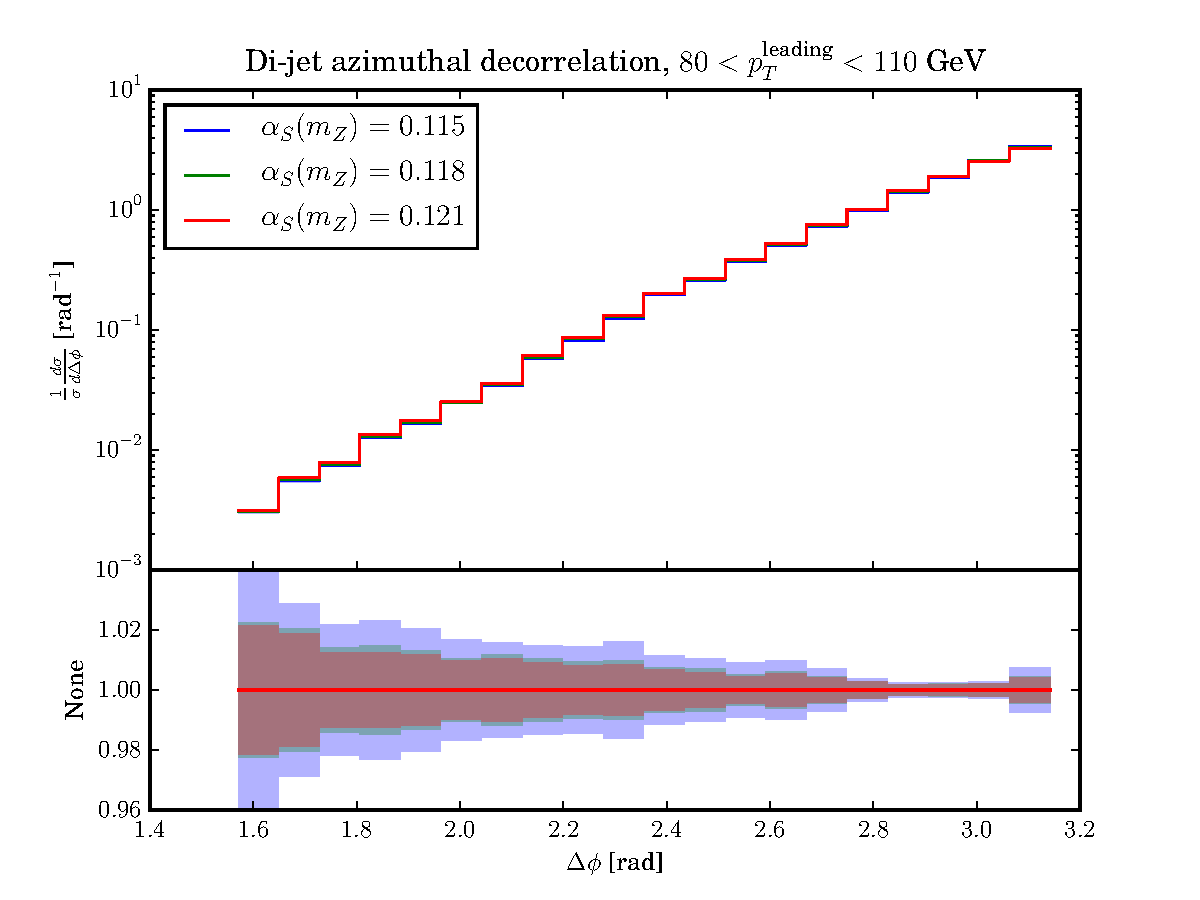
\includegraphics[width=0.49\textwidth]{d01-x01-y01_PDF-errors}
    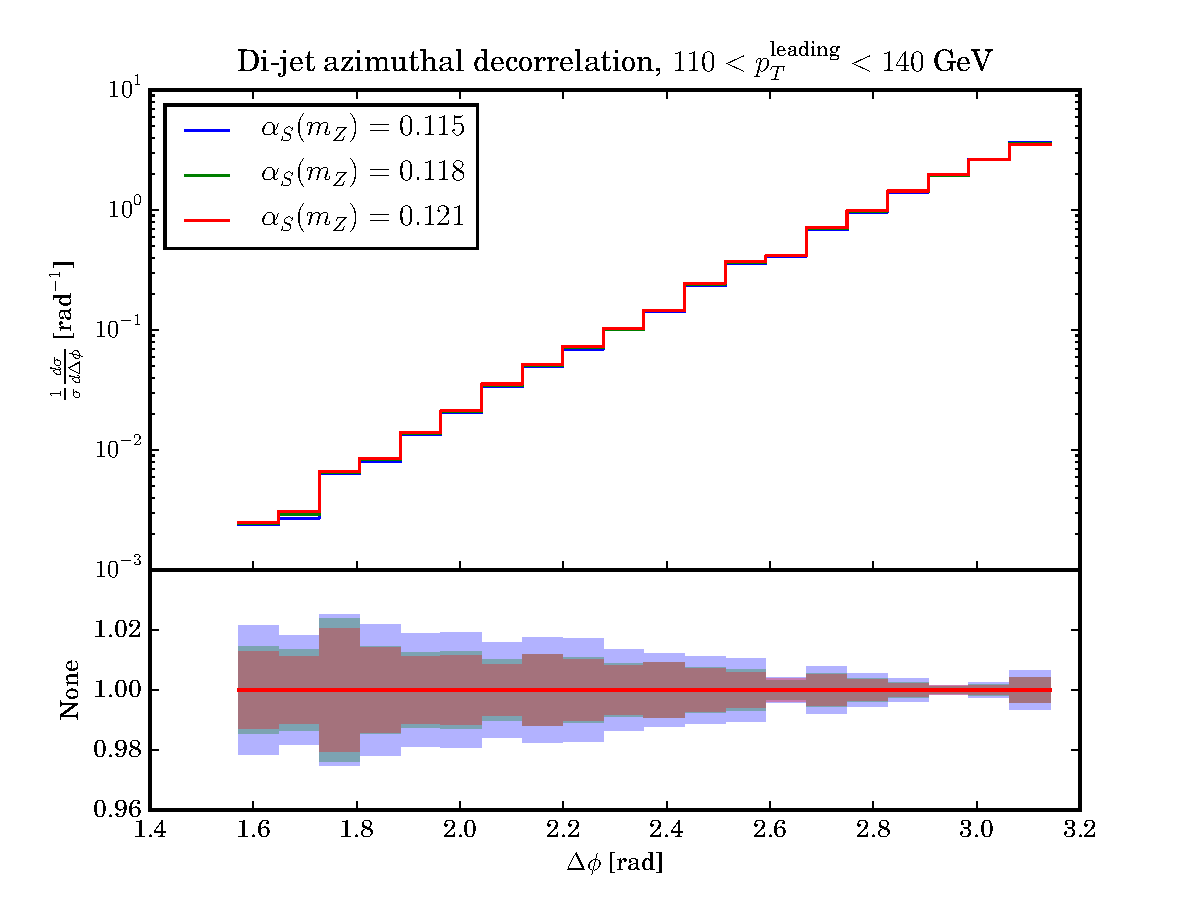
\includegraphics[width=0.49\textwidth]{d02-x01-y01_PDF-errors}
    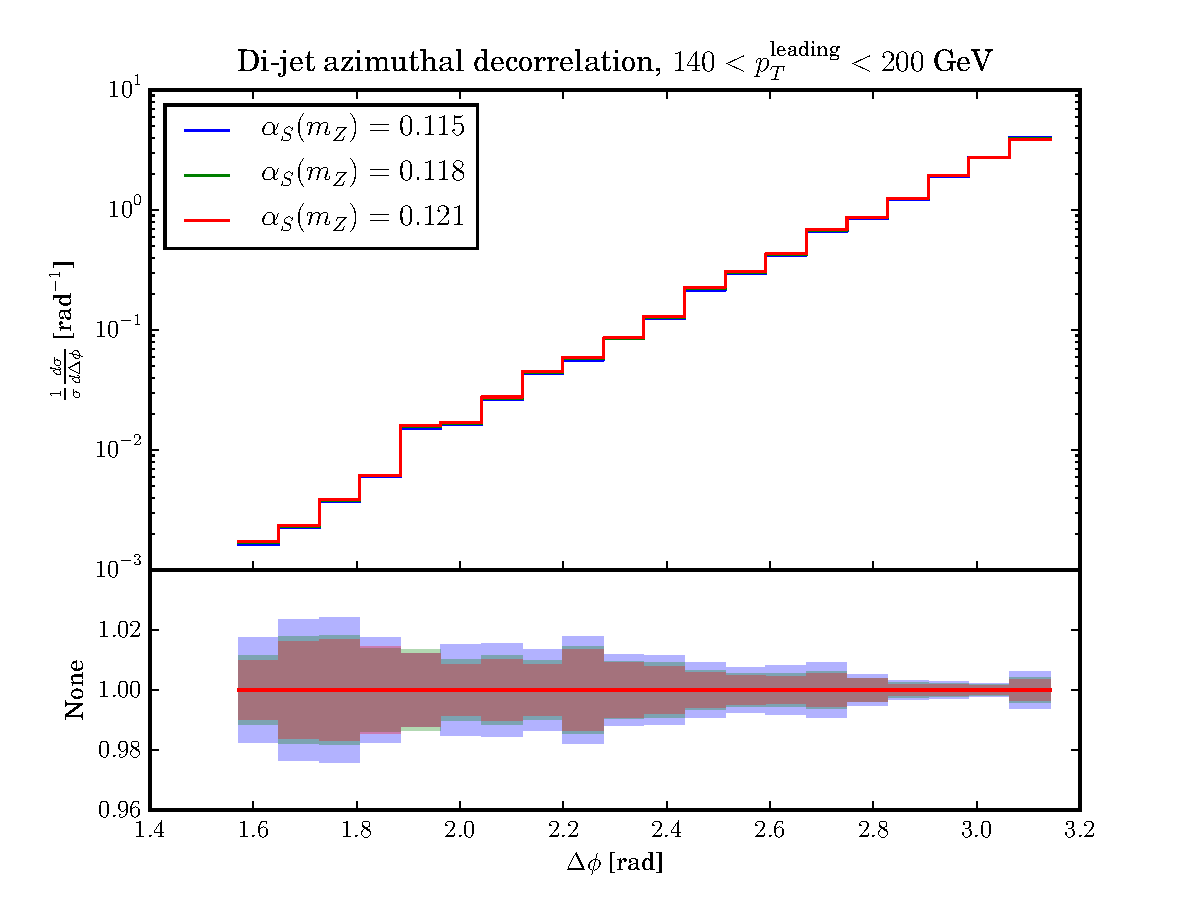
\includegraphics[width=0.49\textwidth]{d03-x01-y01_PDF-errors}
    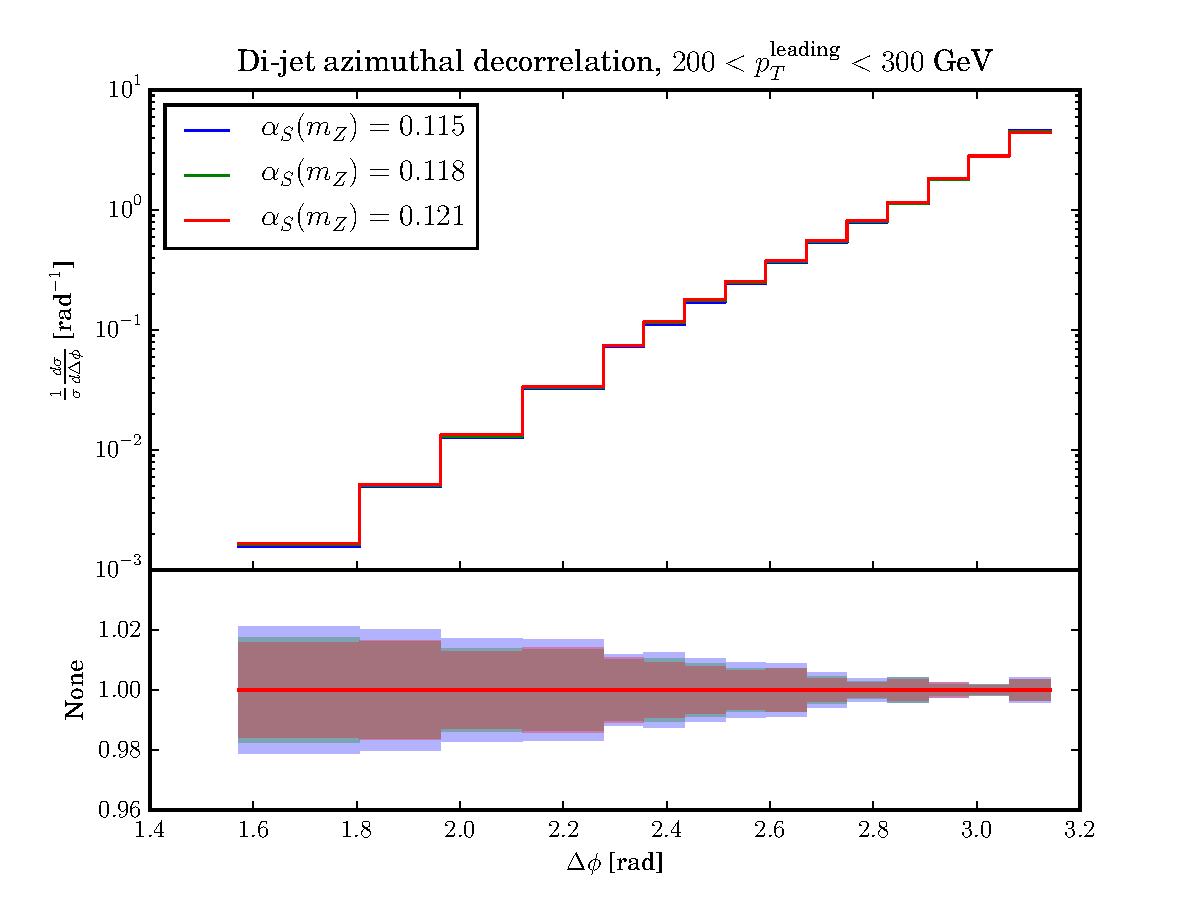
\includegraphics[width=0.49\textwidth]{d04-x01-y01_PDF-errors}
    \caption{PDF errors for the different $\alphas(m_Z)$ values
    in MCatNLO calculations.
    The errors are all of a similar shape, but for $\alphas(m_Z)=0.115$,
    the magnitude of the errors is about \SI{50}{\percent} larger.
    All variations have been calculated with a reweighting,
    where only the hardest emissions is included in the reweighting.}
    \label{fig:pdferrors}
\end{figure}
\section{Fit methodology and result}
Summarise the considerations for the \alphas fit.

\bibliography{refs}
\bibliographystyle{plain}
\end{document}
